\section{Formatowanie}
\label{sec:formatting}

Czcionki tytułu, i~czterech poziomów zagnieżdżeń sekcji powinny odpowiednio przyjąć rozmiar 14, 12, 10, 10, 10 punktów i~być pogrubione (z~wyjątkiem ostatniego poziomu, wyróżnianego kursywą).

\subsection{Podział tekstu}
\label{subsec:textDivision}

Pierwszy akapit sekcji (niezależnie od poziomu ich zagnieżdżenia) występuje z~pominięciem wcięcia, podobnie akapit występujący po ilustracji lub tabeli.

Następujące po nim akapity powinny być wcięte.

\subsubsection{Poziomy sekcji.}
\label{subsubsec:levels}

Jak można zauważyć, nagłówek 3.~i~4. poziomu sekcji należy kończyć kropką \cite{ref:lncs}. Wyłącznie dwa pierwsze poziomy są numerowane. Dalsze zagnieżdżenie skutkuje brakiem numeracji - wymagany sposób formatowania tekstu w~tym przypadku to wlewanie nagłówków w~tej samej linii.

\paragraph{Granice zagnieżdżania.}
\label{par:nestingLimits}

W niniejszym szablonie dopuszcza się możliwość stosowania maksymalnie czterech poziomów zagnieżdżenia, jednak ostatni poziom najczęściej wpływa negatywnie na czytelność tekstu.

\subsubsection{Dzielenie wyrazów.}
\label{subsubsec:wordbreak}

Należy pamiętać o~dzieleniu wyrazów zgodnie z~polską ortografią. W~tym celu, należy stosować łącznik -- pauzę lub półpauzę. Sugeruje się unikanie pauzy w~celu zwiększenia czytelności tekstu.

\subsubsection{Łamanie linii.}
\label{subsubsec:linebreak}

Tekst powinien być wyrównany obustronnie. Część wyrazów w~języku polskim (np. krótkie spójniki) nie może być stosowana na końcu linii. Aby tego uniknąć, należy zastosować skrypt porządkujący tekst lub korzystać ze znaku twardej spacji. Należy zastosować słownikowe reguły dzielenia wyrazów w~celu zwiększenia czytelności tekstu.

\subsubsection{Łamanie stron.}
\label{subsubsec:pagebreak}

Dobrą praktyką, nie zawsze możliwą do realizacji, jest przejście do nowej strony na granicach akapitów i~w~taki sposób, aby w treści akapitu kończącego stronę nie było odwołania do ilustracji/tabeli znajdującego się na kolejnej. Należy unikać kontynuacji niewielkiej części wątku na następnej stronie, szczególnie jeśli jest parzysta (niewidoczna w~trybie czytania dwóch stron naraz).

\subsubsection{Odstępy pionowe.}
\label{subsubsec:verticalSpace}

Nadmierne odstępy pionowe utrudniają odbiór tekstu. Wdrożenie zasady łamania stron może wpłynąć na zwiększenie wspomnianych odstępów. Warto w~takim przypadku rozważyć możliwość przeredagowania tekstu aby umieścić zawartość jeszcze jednego akapitu na stronie.

\subsection{Uzupełnienia treści.}
\label{subsec:additions}

Wśród często stosowanych obiektów urozmaicających treść są tabele i~rysunki. Rozpatrzmy oba przykłady (Rys.~\ref{fig:devop}, Tab.~\ref{tab:styles}).

{
\tikzset{sub/.style = {shape=rectangle, draw, align=center}}
\tikzset{beg/.style = {circle, fill=black}}
\tikzset{end/.style = {circle}}
\tikzset{non/.style = {draw=none}}

\begin{figure}[!h]
	\vspace{-10pt}
	\centering
	\subfloat{
		
\includegraphics[width=12cm]{figure-legend.png}
	}\\
	\subfloat{
	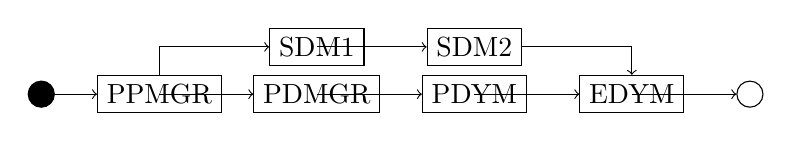
\begin{tikzpicture}[
			every node/.style = sub
		]
		% Nodes
		\node[beg]  (beg) at (-1.5, 0.0) {};
		\node[end]  (end) at ( 7.5, 0.0) {};
		\node         (a) at ( 0.0, 0.0) {PPMGR};
		\node         (b) at ( 2.0, 0.0) {PDMGR};
		\node         (c) at ( 2.0, 0.6) {SDM1};
		\node         (d) at ( 4.0, 0.6) {SDM2};
		\node         (e) at ( 4.0, 0.0) {PDYM};
		\node         (f) at ( 6.0, 0.0) {EDYM};
		% Arrows
		\foreach \from/\to in {beg/a, a/b, a/c, c/d, b/e, e/f, f/end}
			\draw [->] (\from) |- (\to);
		\foreach \from/\to in {d/f}
			\draw [->] (\from) -| (\to);
		\end{tikzpicture}
	}
		\caption{Krótkie podpisy należy wyrównać do środka.}
		\label{fig:devop}
\end{figure}
}


\begin{table}[!h]
	\vspace{-4mm}
	\caption{
		Style wlewania tekstu.
	}
	\begin{center}
		\begin{tabular}{lll}
			\hline
			Typ & Przykład & Styl i~wielkość czcionki\\
			\hline
			Tytuł & {\Large\bfseries Zasady} & 14 punktów, pogrubiona\\
			Sekcja &  {\large\bfseries 1 Wprowadzenie} & 12 punktów, pogrubiona\\
			Podsekcja & {\bfseries 2.1 Podział tekstu} & 10 punktów, pogrubiona\\
			Paragraf & {\bfseries Poziomy sekcji} & 10 punktów, pogrubiona\\
			Podparagraf & {\textit Granice zagnieżdżania} & 10 punktów, kursywa\\
			Zwykły tekst & Nadmierne odstępy pionowe & 10 punktów\\
			Podpis & {\small\textbf{Tab. \ref{tab:styles}.} Style wlewania tekstu} & 9~punktów\\
			\hline
		\end{tabular}
	\end{center}
	\label{tab:styles}
	\vspace{-6mm}
\end{table}

\noindent Zazwyczaj w~tekście anonsujemy, objaśniamy lub komentujemy ilustracje i~tabele. W~ten sposób Czytelnik jest w stanie poznać intencje autora dotyczące prezentacji obiektów urozmaicających w~artykule. Podpis powinien znajdować się powyżej tabeli, ale poniżej rysunku. Powinien także identyfikować zawartość, a~jeśli potrzebne jest obszerniejsze omówienie, to pojawia się ono w~tekście. Należy zwrócić uwagę na dopasowanie rozmiaru obiektów do pozostałej treści strony.

\subsubsection{Wykresy.}
\label{subsubsec:charts}

Korzystając z~tej formy prezentacji informacji, warto pamiętać o~opisaniu osi wykresu, użyciu adekwatnej skali i~typie dostosowanym do rodzaju danych, a~także konsekwencji stylistycznej.

\begin{figure}[!h]
	\centering
	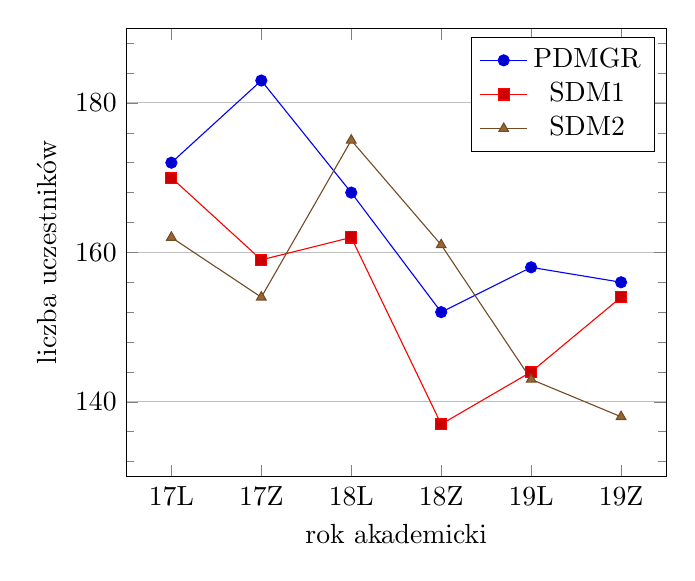
\begin{tikzpicture}
	\begin{axis} [
		minor y tick num = 4,
		ymajorgrids,
		%ybar,
		%%bar width={3pt},
		xtick=data,
		xlabel = {rok akademicki},
		ylabel = {liczba uczestników},
		symbolic x coords = {16L,16Z,17L,17Z,18L,18Z,19L,19Z},
		ymin=130, ymax=190
	]
		\addplot+ coordinates {
			%(16L, 155)
			%(16Z, 159)
			(17L, 172)
			(17Z, 183)
			(18L, 168)
			(18Z, 152)
			(19L, 158)
			(19Z, 156)
		}; \addlegendentry{PDMGR};
		\addplot+ coordinates {
			%(16L, 135)
			%(16Z, 162)
			(17L, 170)
			(17Z, 159)
			(18L, 162)
			(18Z, 137)
			(19L, 144)
			(19Z, 154)
		}; \addlegendentry{SDM1};
		\addplot+[mark=triangle*] coordinates {
			%(16L, 200)
			%(16Z, 115)
			(17L, 162)
			(17Z, 154)
			(18L, 175)
			(18Z, 161)
			(19L, 143)
			(19Z, 138)
		}; \addlegendentry{SDM2};
	\end{axis}
	\end{tikzpicture}
	\caption{Długie podpisy (zajmujące więcej niż jedną linię), należy wyrównać obustronnie. Wielkość czcionek w~opisach obiektów na ilustracjach powinna być zbliżona do wielkości używanej w~podpisie. Obyczaj używania znaczników wynika z~nieczytelności kolorowych wykresów na czarno-białych wydrukach i~kopiach.}
	\label{fig:stats}
	\vspace{-20pt}
\end{figure}

\subsubsection{Wnioskowanie logiczne.}
\label{subsubsec:logic}

Korzysta się z~wielu form prezentacji logicznych wyrażeń: pytania, spostrzeżenia, teorie i~hipotezy, lematy, twierdzenia, dowody i~wnioski, definicje, przykłady, własności i~rozwiązania. Student może je (oszczędnie) stosować, aby uporządkować tok rozumowania.

\begin{claim}
	Dla liczb dodatnich całkowitych a~i~b, jeśli liczba $a^{2}$ jest podzielna przez liczbę $a+b$, to także liczba $b^{2}$ jest podzielna przez $a+b$.
\end{claim}
\begin{proof}
	Zauważmy, że $b^{2} - a^{2} = (b-a)(b+a)$, czyli:

	\begin{equation} \label{eq:formula}
		b^{2} = a^{2} + (b-a)(b+a).
	\end{equation}

	\noindent Skoro liczba $a^{2}$ jest podzielna przez $a+b$, to prawa strona równania (\ref{eq:formula}) również, na podstawie rozdzielności mnożenia względem dodawania, ponieważ jest sumą liczb podzielnych przez $a+b$. \qed
\end{proof}

Należy zwrócić szczególną uwagę na spójność argumentacji i~dostosowanie poziomu szczegółowości wnioskowania do spodziewanego stanu wiedzy odbiorcy artykułu. Sugeruje się zastosowanie krytycznego podejścia do autorskich badań, precyzyjny opis procedury i~środowiska testowego, a~także wnikliwą analizę otrzymanych rezultatów.

\subsubsection{Pseudokod.}
\label{subsubsec:pseudocode}

Zaleca się użycie pseudokodu w~celu przedstawienia zasady działania algorytmu. Należy stosować minimalistyczne podejście w~opisie obiektów, tj.~pomijać numerację dla typów występujących w~tekście wyłącznie jeden raz.

\vspace{-4mm}
\begin{algorithm}
	\renewcommand{\thealgorithm}{} % comment it if multiple algorithms exist
	\caption{Algorytm Euklidesa} \label{alg:euclid}
	\begin{algorithmic}[1]
		\Procedure{NWD}{$a,b$} \Comment{Największy wspólny dzielnik liczb całkowitych a i b}
			\State $r\gets a\bmod b$
			\While{$r\not=0$} \Comment{W przeciwnym przypadku odpowiedź jest trywialna}
				\State $a\gets b$
				\State $b\gets r$
				\State $r\gets a\bmod b$
			\EndWhile \label{alg:euclid:endwhile}
			\State \textbf{return} $b$
		\EndProcedure
	\end{algorithmic}
\end{algorithm}
\vspace{-8mm}

\subsubsection{Cytowanie.}
\label{subsubsec:cite}

Wymaganym stylem cytowania są liczby w nawiasach kwadratowych, uporządkowane według kolejności wystąpienia w~artykule \cite{ref:lncs}, ponieważ stosowanie etykiet lub nazwisk mogłoby wpłynąć negatywnie na czytelność tekstu. Cytowania wielu źródeł powinny być zgrupowane \cite{ref:lncs,ref:latex}, a~wszystkie pozycje literatury - mieć swoje odwołania w tekście.

\subsubsection{Inne konstrukcje.}
\label{subsubsec:others}

Konstrukcje przedstawione powyżej są typowe dla artykułów naukowych i~technicznych. Użycie innych, nietypowych konstrukcji powinno być uzasadnione specyfiką zagadnienia opisywanego w~artykule.
